\begin{figure}[ht]
	\begin{subfigure}[b]{0.32\linewidth}
		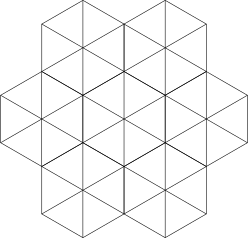
\includegraphics[width=\linewidth]
		{data/synthetic_meshes/hexagonal_tessellation_Dirac_delta_1_v31_f42_wireframe.png}
		\caption{R=1 wireframe}\label{fig:hex.a}
	\end{subfigure}
	\begin{subfigure}[b]{0.32\linewidth}
		\includegraphics[width=\linewidth]
		{data/synthetic_meshes/hexagonal_tessellation_Dirac_delta_1_v31_f42_funcvals_0iter_crop.png}
		\caption{R=1, convolutions 0}\label{fig:hex.b}
	\end{subfigure}
	\begin{subfigure}[b]{0.32\linewidth}
		\includegraphics[width=\linewidth]
		{data/synthetic_meshes/hexagonal_tessellation_Dirac_delta_1_v31_f42_funcvals_2iter_crop.png}
		\caption{R=1, convolutions 2}\label{fig:hex.c}
	\end{subfigure}

	\begin{subfigure}[b]{0.32\linewidth}
		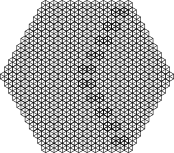
\includegraphics[width=\linewidth]
		{data/synthetic_meshes/hexagonal_tessellation_Dirac_delta_10_v1057_f1986_wireframe.png}
		\caption{R=10 wireframe}\label{fig:hex.d}
	\end{subfigure}
	\begin{subfigure}[b]{0.32\linewidth}
		\includegraphics[width=\linewidth]
		{data/synthetic_meshes/hexagonal_tessellation_Dirac_delta_10_v1057_f1986_funcvals_0iter_crop.png}
		\caption{R=10, convolutions 0}\label{fig:hex.e}
	\end{subfigure}
	\begin{subfigure}[b]{0.32\linewidth}
		\includegraphics[width=\linewidth]{data/synthetic_meshes/hexagonal_tessellation_Dirac_delta_10_v1057_f1986_funcvals_200iter_crop.png}
		\caption{R=10, convolutions 200}\label{fig:hex.f}
	\end{subfigure}
	\caption[Six views, comparing two differently sized hexagonal tessellations]{Comparison of two differently sized hexagonal tessellations, generated with parameters R set to 1 and 10: (a) R=1 in wireframe (b) R=1 colored by function value before convolving the filter (c) R=1 colored by function value after convolving the filter once (d) R=10 in wireframe (e) R=10 colored by function value before convoving the filter (f) R=10 colored by function value after convolving the filter 200 times.}
	\label{fig:hex}
\end{figure}
\todoCitation{}
